Dans cette version adaptée du biathlon, les élèves ont à parcourir, en courant, 4 grands tours tracés avec des plots sur un stade comme dans la figure ci-dessous. À l'issue de chacun des 3 premiers tours, ils se présentent au pas de tir et lancent 3 balles sur des cibles. S'ils atteignent 3 fois leur cible, ils n'ont pas de pénalité et repartent pour le grand tour suivant. En revanche, pour chaque lancer manqué, ils doivent effectuer un petit tour avant de repartir sur le grand tour.

Pour chaque élève on mesure la durée mise pour faire un parcours complet (grands tours + lancers + petits tours de pénalité le cas échéant). L'objectif est de mettre le moins de temps possible pour effectuer le parcours complet.

\begin{center}
  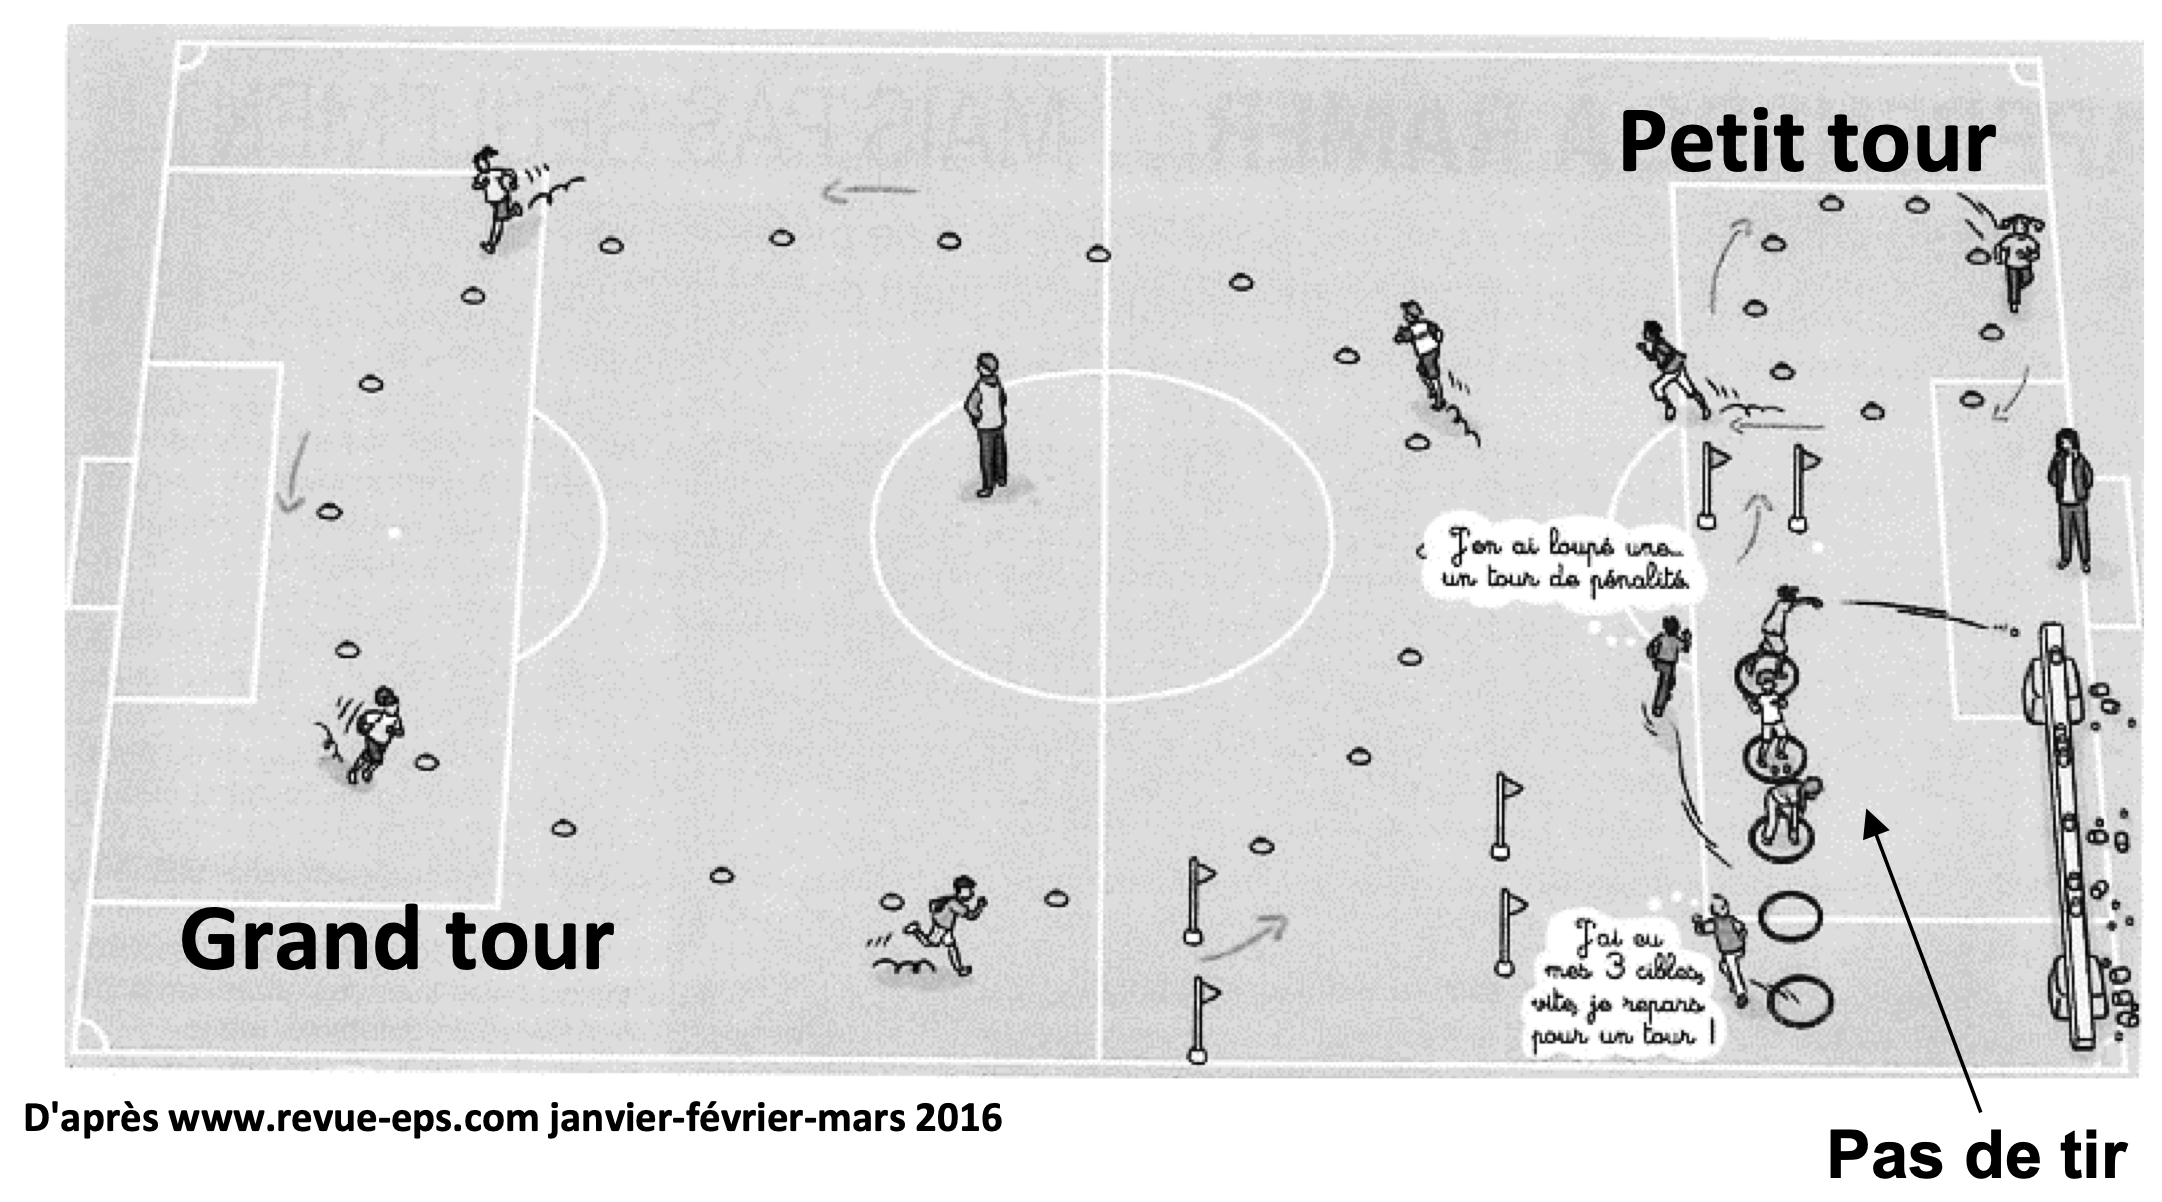
\includegraphics[width=.8\textwidth]{2022-g1-ex1-img1.png}	
\end{center}


\section*{Partie 1}

Dans cette partie, les élèves s'entraînent à la course sur le grand tour, sans effectuer de lancer de balles.

\begin{enumerate}
  \item Pour un élève de CE1, la longueur du grand tour est de $250 \mathrm{~m}$.
  
  \begin{enumerate}
  \item On considère un élève, qui effectue les 4 tours en 10 minutes. Quelle est sa vitesse moyenne de course, en mètre par minute ?
  \item Un autre élève a couru les 4 tours à la vitesse moyenne de $150 \mathrm{~m} / \mathrm{min}$. Déterminer sa vitesse moyenne en kilomètre par heure.
  \end{enumerate}

  \item Dans le tableau ci-dessous, les longueurs d'un grand tour pour des élèves de CM1 et de CM2 sont données, ainsi que les temps de course pour effectuer 4 grands tours, de deux élèves (un en $\mathrm{CM} 1$ et un en $\mathrm{CM} 2$ ).
 
 
 \medskip
\begin{tabular}{|c|c|c|}
\hline
\bfseries Elève & \bfseries Longueur de 1 grand tour & \bfseries Temps de course pour 4 grand tours \\
\hline
Elève de CM1 & $400 \mathrm{~m}$ & 9 minutes et 30 secondes \\
\hline
Élève de CM2 & $500 \mathrm{~m}$ & 11 minutes et 8 secondes \\
\hline
\end{tabular}

\medskip
Déterminer la vitesse moyenne (en mètre par minute, arrondie à l'unité) de chacun de ces deux élèves, lorsqu'ils ont réalisé les 4 grands tours.
\end{enumerate}


\section*{Partie 2}

Dans cette partie, des élèves de CE1 font l'épreuve de biathlon dans sa totalité :

Les 4 grands tours + les 3 épreuves de lancers de 3 balles + les éventuels tours de pénalité.

\medskip
On rappelle que pour un élève de CE1, la longueur du grand tour est de $250 \mathrm{~m}$.

\medskip
\begin{enumerate}
  \item La longueur du tour de pénalité est de $20 \mathrm{~m}$.
  
  \begin{enumerate}
  	\item Sachant que le tour de pénalité forme un cercle, déterminer son rayon. Arrondir au centimètre.
  	\item Un élève de CE1, qui court à la vitesse moyenne de $150 \mathrm{~m} / \mathrm{min}$, prend le départ de l'épreuve. On suppose que pour effectuer 3 lancers, il passe, à chaque fois, 30 secondes sur le pas de tir.\\
Quelle sera la durée totale que met cet élève pour réaliser le parcours complet, s'il ne rate aucune cible au premier tour et qu'il rate une cible au 2\up{e} tour puis deux cibles au 3\up{e} tour ? Donner la réponse en minutes et secondes.

	\end{enumerate}

  \item Le professeur des écoles souhaite aider ses élèves à développer une stratégie pour améliorer leurs résultats. II relève les performances d'un même élève de CE1 qui fait 3 fois l'épreuve de biathlon dans sa totalité en modifiant certains paramètres à chaque essai. Dans le tableau ci-dessous, $V_{\text {moy }}$ est la vitesse moyenne de cet élève sur les périodes de course (4 grands tours + éventuels tours de pénalités).


\begin{center}
  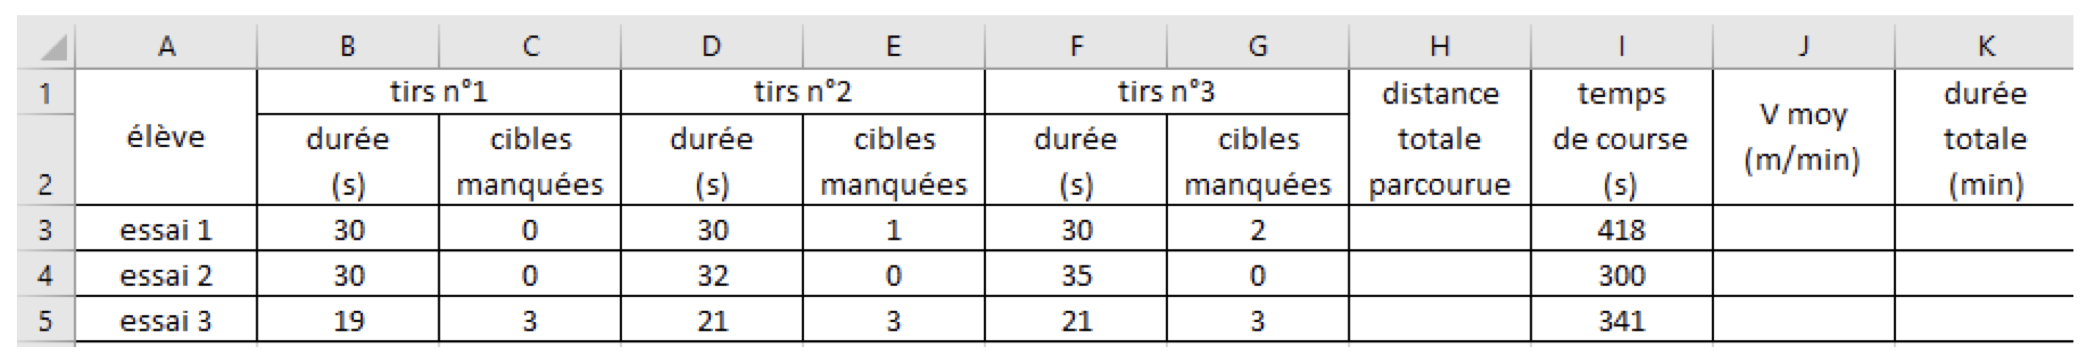
\includegraphics[width=\linewidth]{2022-g1-ex1-img2.png}	
\end{center}

	\begin{enumerate}
		\item La formule saisie en H3 puis recopiée vers le bas est
$$
=1000+(C 3+E 3+G 3)^{*} 20 \text {. }
$$
Expliquer le terme $(C 3+E 3+G 3)^{*} 20$ dans le contexte de l'exercice.

        \item Donner une formule qui pourra être introduite dans la cellule J3, de telle sorte qu'elle puisse être recopiée vers le bas pour effectuer le calcul pour les autres essais.
        \item Donner une formule qui pourra être introduite dans la case \og{} durée totale \fg{} K3, de telle sorte qu'elle puisse être recopiée vers le bas pour effectuer le calcul pour les autres essais.

Après calculs, on obtient le tableau complet ci-dessous :

\begin{center}
  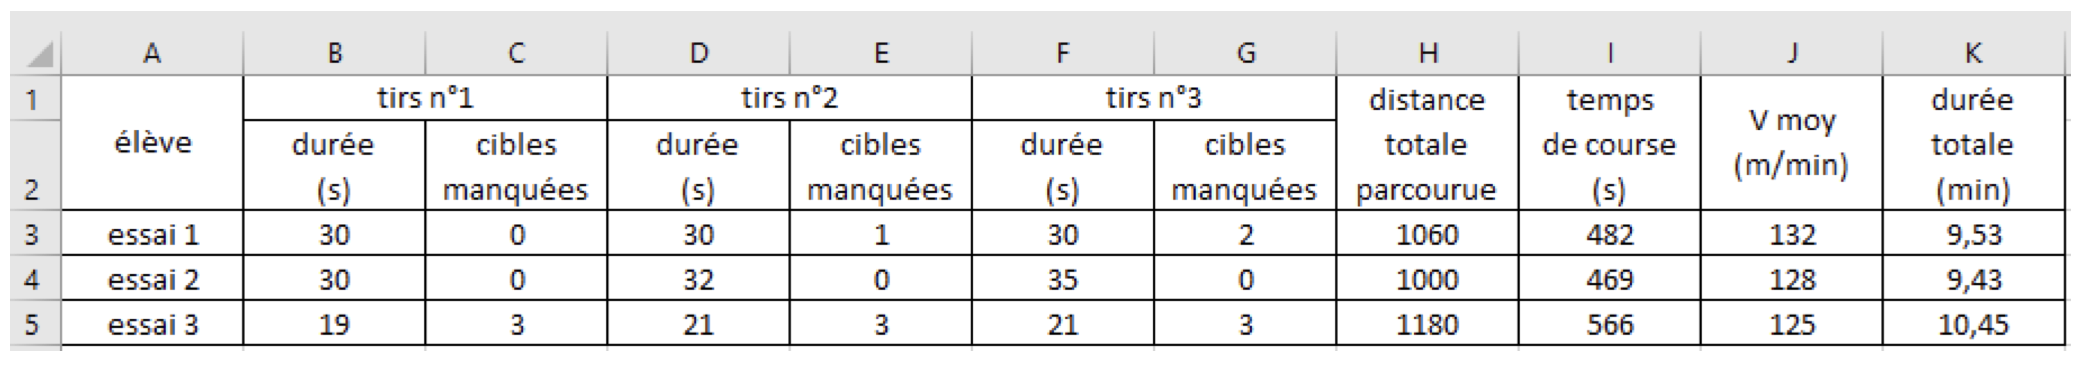
\includegraphics[width=\linewidth]{2022-g1-ex1-img3.png}	
\end{center}

		\item Interpréter le tableau pour déterminer ce que l'élève a modifié entre l'essai 2 et l'essai $3 .$
		\item Si on analyse les performances de l'élève aux essais 2 et 3, quelle hypothèse ce tableau permet-il de faire du point de vue des stratégies à adopter ?
		\end{enumerate}
		
\end{enumerate}
